% !TeX spellcheck = en_GB
\documentclass[10pt]{beamer}
\usetheme{CambridgeUS}
%\usetheme{Boadilla}
\definecolor{myred}{RGB}{163,0,0}
%\usecolortheme[named=blue]{structure}
\usecolortheme{dove}
\usefonttheme[]{professionalfonts}
\usepackage[english]{babel}
\usepackage{amsmath,amsfonts,amssymb}
\usepackage{xcolor}
\usepackage{bm}
\usepackage{gensymb}
\usepackage{verbatim} 
\usepackage{paratype}
\usepackage{mathpazo}
\usepackage{listings}
\lstset{language=Python}

\usepackage{tikz}
\usetikzlibrary{matrix}

% Number theorem environments
\setbeamertemplate{theorem}[ams style]
\setbeamertemplate{theorems}[numbered]

% Reset theorem-like environments so that each is numbered separately
\usepackage{etoolbox}
\undef{\definition}
\theoremstyle{definition}
\newtheorem{definition}{\translate{Definition}}
\newtheorem{Fact}{\translate{Fact}}

% Change colours for theorem-like environments
\definecolor{mygreen1}{RGB}{0,96,0}
\definecolor{mygreen2}{RGB}{229,239,229}
\setbeamercolor{block title}{fg=white,bg=mygreen1}
\setbeamercolor{block body}{fg=black,bg=mygreen2}



\alt<presentation>
{\lstset{%
  basicstyle=\footnotesize\ttfamily,
  commentstyle=\slshape\color{green!50!black},
  frame = single,  
  keywordstyle=\bfseries\color{blue!50!black},
  identifierstyle=\color{blue},
  stringstyle=\color{orange},
  %escapechar=\#,
  showstringspaces = false,
  showtabs = false,
  tabsize = 2,
  emphstyle=\color{red}}
}
{
  \lstset{%
    basicstyle=\ttfamily,
    keywordstyle=\bfseries,
    commentstyle=\itshape,
    escapechar=\#,
    showtabs = false,
	tabsize = 2,
    emphstyle=\bfseries\color{red}
  }
} 

\title{R401: Statistical and Mathematical Foundations \bigskip}
\subtitle{\textcolor{myred}{Unconstrained Optimization. Static Optimization with Equality Constraints. Lagrange Multipliers}}
\author{Andrey Vassilev}

\date{}

\AtBeginSection{\frame{\usebeamerfont{section title}\centering\insertsection}}

\begin{document}
\maketitle

\begin{frame}[fragile]
\frametitle{General Principles and Caveats for the Optimization Module}
\begin{itemize}
\item Emphasis on practicality over rigour
\item Consequently, algorithmic approach and ``recipes'' rather than proofs
\item Also, existence and relevant properties of various objects are often implicitly assumed
\item Pathologies and mathematical peculiarities discussed only in special cases
\end{itemize}
\end{frame}

\begin{frame}[fragile]
\frametitle{Lecture Contents}
\tableofcontents
\end{frame}

\begin{section}{Warm-up: Basic Unconstrained Optimization in $ \mathbb{R}^1 $}\label{sec:R1}

\begin{frame}[fragile]
\frametitle{Warm-up: Basic Unconstrained Optimization in $ \mathbb{R}^1 $}

\begin{Fact}
For a function $ f: \mathbb{R} \rightarrow \mathbb{R} $ differentiable at a point $ x $, a necessary condition for a local extreme point (i.e. a maximum or a minimum) at $ x $ is \[ f'(x) = 0. \]
\end{Fact}
\bigskip

\begin{example} %{Example}
If $ f(x) = ax^2 + bx + c $, then $ f'(x) = 2ax + b $ and the condition $ f'(x)=0 $ yields the familiar $ x=-\frac{b}{2a} $ (recall your high-school days). Depending on the sign of $ a $, this is a maximum or a minimum (What is the relationship?).
\end{example}\bigskip

\begin{example} %{Example}
If $ f(x) = x^3 $, then $ f'(x)=3x^2 $ and $ f'(x)=0 \Rightarrow x=0$.

Does the function attain a maximum or a minimum at $ x=0 $?
\end{example}
\end{frame}

\begin{frame}[fragile]
\frametitle{Warm-up: Basic Unconstrained Optimization in $ \mathbb{R}^1 $}
\begin{figure}
\centering
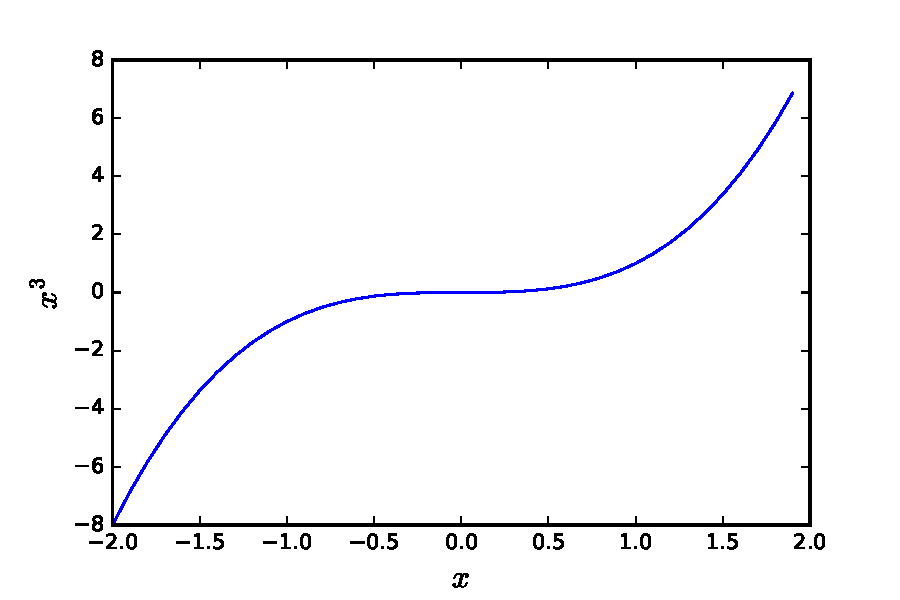
\includegraphics[width=0.9\linewidth]{cubicfun}
\label{fig:cubicfun}
\end{figure}
\end{frame}

\begin{frame}[fragile]
\frametitle{Warm-up: Basic Unconstrained Optimization in $ \mathbb{R}^1 $}
\addtocounter{theorem}{-1}
\begin{example}[cont.]
The answer is ``neither''! The point $ x=0 $ is not a local extreme point of $ f(x)=x^3 $.\medskip

This illustrates the pitfalls of using necessary conditions -- they supply only candidates that need to be checked further.
\end{example}

The above examples generalize in the following manner:
\begin{Fact}
Let a function $ f $ be $ n $ times differentiable at a point $ x $ and 
\[ f'(x)=f''(x)=\ldots=f^{(n-1)}(x)=0,\qquad f^{(n)}\neq 0. \] \vskip -5pt
\begin{enumerate}
\item If $ n $ is odd, the point $ x $ is not an extreme point of $ f(x) $.
\item If $ n $ is even and $ f^{(n)}(x)>0 $, the point $ x $ is a minimum.
\item If $ n $ is even and $ f^{(n)}(x)<0 $, the point $ x $ is a maximum.
\end{enumerate}
\label{fc:SCsR1}
\end{Fact}
\end{frame}

\end{section}

\begin{section}{Unconstrained Optimization in $ \mathbb{R}^n $}\label{sec:Rn}

\begin{frame}[fragile]
\frametitle{Unconstrained Optimization in $ \mathbb{R}^n $}
\framesubtitle{Necessary conditions}
\begin{Fact}
For a function $ f: \mathbb{R}^n \rightarrow \mathbb{R}$, differentiable at a point $ \mathbf{x} $, a necessary condition for $ \mathbf{x} $ to be a local extreme point is \[ f'(\mathbf{x}) = \mathbf{0}, \]
where \[ \mathbf{x} = \left( \begin{array}{c}
x_1 \\
x_2\\
\vdots \\
x_n
\end{array}\right),~\mathbf{0} = \left( \begin{array}{c}
0 \\
0 \\
\vdots \\
0
\end{array}\right)\text{ and }  f'(\mathbf{x})  = \left( \begin{array}{c}
\dfrac{\partial f(x_1,\ldots,x_n)}{\partial x_1}\\
\vdots \\
\dfrac{\partial f(x_1,\ldots,x_n)}{\partial x_n}
\end{array}\right)(= \nabla f(\mathbf{x})) \]
\label{fc:NCsRn}
\end{Fact}

\textbf{Note:} A point where the gradient of a function $ f $ vanishes is called a \emph{critical point} or a \emph{stationary point}. This also applies to functions on $ \mathbb{R}^1 $.
\end{frame}

\begin{frame}[fragile]
\frametitle{Unconstrained Optimization in $ \mathbb{R}^n $}
\begin{example}
\[ f(x,y) = x^2 +2y^2-3x+xy \]
\[ \frac{\partial f}{\partial x} = 2x-3+y=0\quad \Rightarrow \quad x=\frac{3-y}{2} \]
\[ \frac{\partial f}{\partial y} = 4y+x = 0\quad \Rightarrow \quad y = -\frac{x}{4}\]
\[ x=\frac{12}{7},~y=-\frac{3}{7} \]
\label{ex:locminR2}
\end{example}
\end{frame}

\begin{frame}[fragile]
\frametitle{Unconstrained Optimization in $ \mathbb{R}^n $}
\begin{figure}
\centering
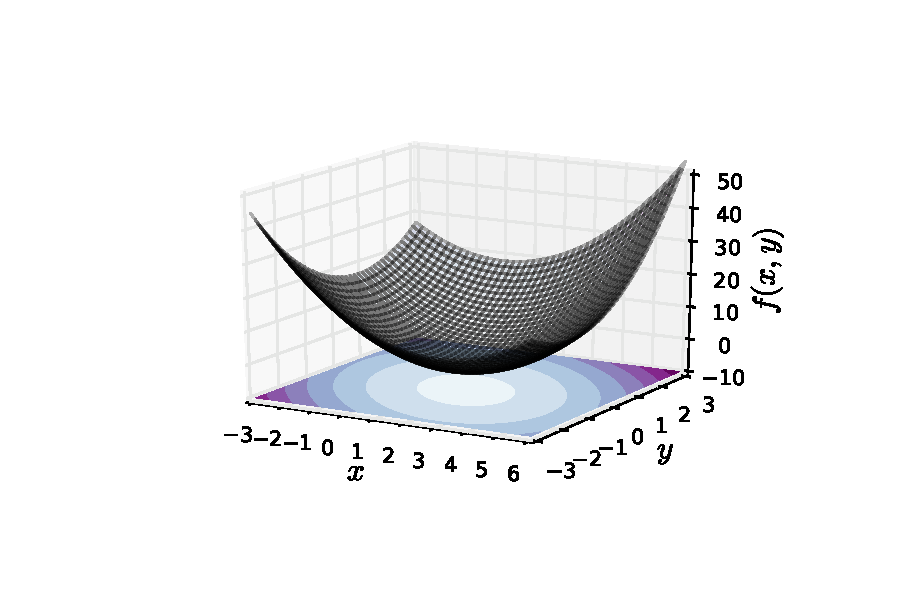
\includegraphics[width=0.9\linewidth]{quadformplot}
\label{fig:quadformplot}
\end{figure}
\end{frame}

\begin{frame}[fragile]
\frametitle{Unconstrained Optimization in $ \mathbb{R}^n $}
The necessity of the condition $  f'(\mathbf{x}) = \mathbf{0} $ has implications that are similar to the univariate case:

\begin{example}
Consider the function $ f(x,y) = x^2 - y^2 $. The NCs yield the following candidate: \[ \frac{\partial f}{\partial x} = 2x = 0\quad \Rightarrow \quad x=0, \]
\[ \frac{\partial f}{\partial y} = -2y = 0\quad \Rightarrow \quad y = 0.\] \bigskip

Let's look at the graph of the function in a neighbourhood of the point $ (0,0)' $.
\label{ex:saddle}
\end{example}
\end{frame}

\begin{frame}[fragile]
\frametitle{Unconstrained Optimization in $ \mathbb{R}^n $}
\begin{figure}
\centering
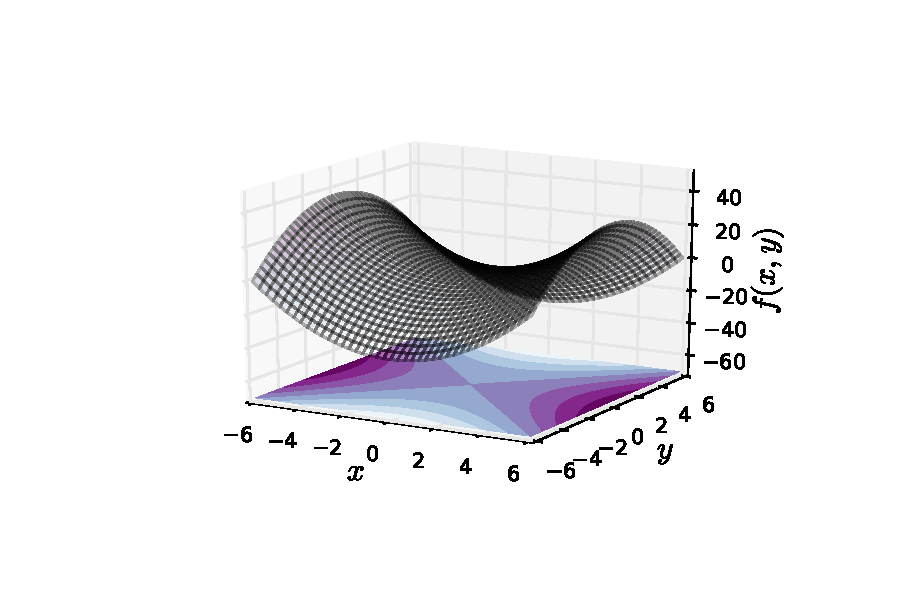
\includegraphics[width=0.9\linewidth]{saddlepoint}
\label{fig:saddlepoint}
\end{figure}
\end{frame}

\begin{frame}[fragile]
\frametitle{Unconstrained Optimization in $ \mathbb{R}^n $}
\addtocounter{theorem}{-1}
\begin{example}[cont.]
The critical point $ \mathbf{x} = (0,0)' $ is an example of a \emph{saddle point}. The function $ f $ (obviously) does not attain an extremum at $ \mathbf{x} $.
\end{example}\bigskip

Example \ref{ex:saddle} illustrates the need to refine the approach for checking candidate points in the $ n $-dimensional case. To this end, we have to review several concepts. \bigskip

A symmetric square matrix $ A $ is called \emph{positive semidefinite} if, for any vector $ \mathbf{x} $, we have \[ \mathbf{x'} A \mathbf{x} \geq 0. \]

If the inequality is strict for any non-zero vector $ \mathbf{x} $, the matrix is called \emph{positive definite}.

Similarly, a symmetric square matrix $ A $ is called \emph{negative semidefinite} if, for any vector $ \mathbf{x} $, we have  $ \mathbf{x'} A \mathbf{x} \leq 0 $, and \emph{negative definite} in case of strict inequality for $ \mathbf{x} \neq \mathbf{0}$.
\end{frame}

\begin{frame}[fragile]
\frametitle{Unconstrained Optimization in $ \mathbb{R}^n $}
Incidentally, for a given square symmetric matrix $ A $, the function
$ Q(\mathbf{x}) = \mathbf{x'} A \mathbf{x}$ is called a \emph{quadratic form}. Quadratic forms are also referred to as ``positive/negative (semi)definite'', depending on the properties of the respective matrix.\bigskip

Recall that, for an $ n \times n $ matrix $ A $, a \emph{principal minor} of order $ k $ ($ 1\leq k \leq n $), denoted by $ \Delta_k $, is the determinant of the submatrix obtained by deleting $ n-k $ rows of the matrix and the correspondingly numbered columns, e.g.

\[ 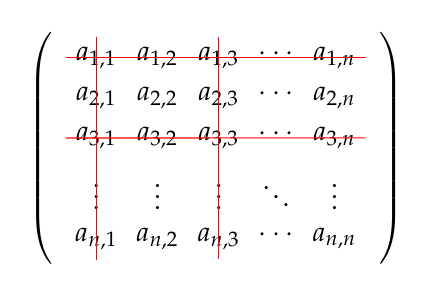
\begin{tikzpicture}
     \matrix (mat)[matrix of math nodes,left delimiter={(},right delimiter={)}]
      {%
		a_{1,1}  &  a_{1,2}  &  a_{1,3}  &  \cdots  &  a_{1,n} \\
		a_{2,1 } &  a_{2,2}  &  a_{2,3}  &  \cdots  &  a_{2,n} \\
		a_{3,1}  &  a_{3,2}  &  a_{3,3}  &  \cdots  &  a_{3,n} \\
		\vdots   &  \vdots   &  \vdots   &  \ddots  &  \vdots \\
		a_{n,1}  &  a_{n,2}  &  a_{n,3}  &  \cdots  &  a_{n,n} \\
      }; \pause
      \draw[red](mat-1-1.west) -- (mat-1-5.east);
      \draw[red](mat-3-1.west) -- (mat-3-5.east);
      \draw[red](mat-1-1.north) -- (mat-5-1.south);
      \draw[red](mat-1-3.north) -- (mat-5-3.south);
\end{tikzpicture}
\]

\textbf{Note:} The notation $ \Delta_k $ does not identify a unique  principal minor of order $ k $.
\end{frame}

\begin{frame}[fragile]
\frametitle{Unconstrained Optimization in $ \mathbb{R}^n $}
The $ k $-th \emph{leading principal minor} of a matrix $ A $ ($ 1\leq k \leq n $), denoted by $ D_k $, is the determinant of the submatrix \[  \begin{pmatrix}
a_{1,1} & a_{1,2} & \cdots & a_{1,k}\\
a_{2,1} & a_{2,2} & \cdots & a_{2,k}\\
\vdots&\vdots& \ddots& \vdots\\
a_{k,1} & a_{k,2} & \cdots & a_{k,k}
\end{pmatrix} , \]
i.e. the principal minor obtained by deleting the last $ n-k $ rows and columns and, respectively, keeping the first $ k $.

\end{frame}

\begin{frame}[fragile]
\frametitle{Unconstrained Optimization in $ \mathbb{R}^n $}
\begin{Fact}[Sylvester's criterion]
Let $ A $ be a symmetric matrix. Then:
\begin{enumerate}
\item $ A $ is positive definite if and only if $ D_k >0,~k=1,\ldots,n $.
\item $ A $ is positive semidefinite if and only if $ \Delta_k \geq 0 $ for all principal minors of order $ k = 1,\ldots,n $.
\item $ A $ is negative definite if and only if $ (-1)^k D_k >0,~k=1,\ldots,n $.
\item $ A $ is negative semidefinite if and only if $ (-1)^k \Delta_k \geq 0 $ for all principal minors of order $ k = 1,\ldots,n $.
\end{enumerate}
\label{fc:Sylvester}
\end{Fact}

Note that the necessary and sufficient conditions for ``semidefiniteness'' involve all principal minors (and hence are cumbersome to check), not just the leading principal minors.
\end{frame}

\begin{frame}[fragile]
\frametitle{Unconstrained Optimization in $ \mathbb{R}^n $}
Let a function $ f(\mathbf{x})=f(x_1,\ldots,x_n) $ be twice differentiable. The matrix of second partial derivatives, evaluated at a point $ \mathbf{x} $, i.e. \[ \begin{pmatrix}
\dfrac{\partial^2 f(\mathbf{x})}{\partial x_1^2 } & \dfrac{\partial^2 f(\mathbf{x})}{\partial x_1 \partial x_2} & \cdots & \dfrac{\partial^2 f(\mathbf{x})}{\partial x_1 \partial x_n}\\[3ex]
\dfrac{\partial^2 f(\mathbf{x})}{\partial x_2\partial x_1 } & \dfrac{\partial^2 f(\mathbf{x})}{\partial x_2^2} & \cdots & \dfrac{\partial^2 f(\mathbf{x})}{\partial x_2 \partial x_n}\\[3ex]
\cdots & \cdots & \ddots & \cdots \\[3ex]
\dfrac{\partial^2 f(\mathbf{x})}{\partial x_n \partial x_1 } & \dfrac{\partial^2 f(\mathbf{x})}{\partial x_n \partial x_2 } & \cdots & \dfrac{\partial^2 f(\mathbf{x})}{\partial x_n^2}
\end{pmatrix} \] is called the \emph{Hessian (matrix)} of $ f $ at $ \mathbf{x} $.
\end{frame}

\begin{frame}[fragile]
\frametitle{Unconstrained Optimization in $ \mathbb{R}^n $}
\begin{itemize}
\item The Hessian is denoted $ \mathbf{f''(x)} $. \bigskip
\item The Hessian is symmetric. \bigskip
\item Sometimes the partial derivative $ \dfrac{\partial^2 f(\mathbf{x})}{\partial x_i \partial x_j} $ is written as $ f''_{ij}(\mathbf{x}) $. \bigskip
\item A leading principal minor of order $ k $ of the Hessian is denoted $ D_k(\mathbf{x}) $. \bigskip
\item An arbitrary principal minor of order $ k $ of the Hessian is denoted $ \Delta_k(\mathbf{x}) $.
\end{itemize}

\end{frame}

\begin{frame}[fragile]
\frametitle{Unconstrained Optimization in $ \mathbb{R}^n $}
\begin{Fact}
Let a (twice) differentiable function $ f: \mathbb{R}^n \rightarrow \mathbb{R} $ have a critical point at $ \mathbf{x^*} $.
\begin{enumerate}
\item If the Hessian  $ \mathbf{f''(x^*)} $ is positive definite or, equivalently, $ D_k(\mathbf{x^*})>0,~k=1,\ldots,n $, then $ \mathbf{x^*} $ is a \emph{local minimum point}.
\item If the Hessian  $ \mathbf{f''(x^*)} $ is negative definite or, equivalently, $ (-1)^k D_k(\mathbf{x^*})>0,~k=1,\ldots,n $, then $ \mathbf{x^*} $ is a \emph{local maximum point}.
\item If $ D_n(\mathbf{x^*})\neq 0 $ and neither 1) nor 2) is satisfied, then $ \mathbf{x^*} $ is a \emph{saddle point}.
\end{enumerate}
\label{fc:ScsRn}
\end{Fact}
\end{frame}

\begin{frame}[fragile]
\frametitle{Unconstrained Optimization in $ \mathbb{R}^n $}
\begin{Fact}
Let a (twice) differentiable function $ f: \mathbb{R}^n \rightarrow \mathbb{R} $ have an extreme point at $ \mathbf{x^*} $.
\begin{enumerate}
\item If $ \mathbf{x^*} $ is a local minimum point, then the Hessian  $ \mathbf{f''(x^*)} $ is positive semidefinite or, equivalently, $ \Delta_k(\mathbf{x^*})\geq 0$ for all principal minors of order $ k=1,\ldots,n $.
\item If $ \mathbf{x^*} $ is a local maximum point, then the Hessian  $ \mathbf{f''(x^*)} $ is negative semidefinite or, equivalently, $ (-1)^k \Delta_k(\mathbf{x^*})\geq 0$ for all principal minors of order $ k=1,\ldots,n $.
\end{enumerate}
\label{fc:NcsRn}
\end{Fact}
\end{frame}

\begin{frame}[fragile]
\frametitle{Unconstrained Optimization in $ \mathbb{R}^n $}
\begin{example}[Verification of Example \ref{ex:locminR2}] Recall that:
\[ f(x,y) = x^2 +2y^2-3x+xy \]
\[ \frac{\partial f}{\partial x} = 2x-3+y,\quad \frac{\partial f}{\partial y} = 4y+x.\]
We now have:
\[ \frac{\partial^2 f}{\partial x^2} = 2, \quad \frac{\partial^2 f}{\partial y^2} = 4,\quad \frac{\partial^2 f}{\partial x \partial y} = 1, \quad  \frac{\partial^2 f}{\partial y \partial x } = 1. \]

\[ D_1 = \det (2) = 2>0, \quad D_2 = \det \begin{pmatrix}
2 & 1\\
1 & 4
\end{pmatrix} = 2 \cdot 4 - 1 \cdot 1 = 7 > 0. \]

Since $ D_1>0,~D_2>0 $, the critical point $ x=\frac{12}{7},~y=-\frac{3}{7} $ is a minimum.
\label{ex:locminR2cont}
\end{example}

%\textbf{Homework:} Apply the same procedure to Example \ref{ex:saddle}.
\end{frame}
\end{section}


\begin{section}{Static Optimization with Equality Constraints. Lagrange Multipliers}\label{sec:Lagr}

\begin{frame}[fragile]
\frametitle{Static Optimization with Equality Constraints}
\framesubtitle{Formulation}
Now we look at problems of the form
\begin{equation}
f(x_1,\ldots,x_n)\rightarrow \min (\max)
\label{eq:obj}
\end{equation}
s.t.
\begin{equation}
\begin{array}{l l l}
g_1(x_1,\ldots,x_n) = b_1\\
g_2(x_1,\ldots,x_n) = b_2\\
\cdots \\
g_m(x_1,\ldots,x_n) = b_m\\
\end{array}
\label{eq:constr}
\end{equation}
where $ m<n $. (Can you explain the last requirement?) \bigskip

\textbf{Note:} In what follows, all required properties of the objects in \eqref{eq:obj} and \eqref{eq:constr} like differentiability are implicitly assumed.
\end{frame}

\begin{frame}[fragile]
\frametitle{Static Optimization with Equality Constraints}
\framesubtitle{Formulation}
Using vector notation for compactness, the objective function is:
\[ f(\mathbf{x}) \rightarrow \min (\max) \]
We introduce
\[ \mathbf{g}(\mathbf{x}):= (g_1(\mathbf{x}),\ldots,g_m(\mathbf{x}))',\quad \mathbf{b} = (b_1,\ldots,b_m)' \]
and the constraints are written as 
\[ \mathbf{g}(\mathbf{x})=\mathbf{b}. \]
\end{frame}

\begin{frame}[fragile]
\frametitle{Static Optimization with Equality Constraints}
\framesubtitle{The Lagrangian}
The standard approach to solving \eqref{eq:obj}-\eqref{eq:constr} starts by defining a \emph{Lagrangian}:

\[ \mathcal{L}(\mathbf{x}) = f(\mathbf{x}) - \lambda_1 (g_1(\mathbf{x})-b_1) - \cdots - \lambda_m (g_m(\mathbf{x})-b_m). \]\bigskip

The numbers $ \lambda_1,\ldots,\lambda_m $ are called \emph{Lagrange multipliers}.\bigskip

This can also be written in vector notation:
\[ \mathcal{L}(\mathbf{x}) = f(\mathbf{x}) - \boldsymbol{\lambda}' (\mathbf{g}(\mathbf{x})-\mathbf{b}) , \] 
where $ \boldsymbol{\lambda }= (\lambda_1,\ldots,\lambda_m)' $ is the vector of Lagrange multipliers.
\end{frame}

\begin{frame}[fragile]
\frametitle{Static Optimization with Equality Constraints}
We can use the Lagrangian to produce necessary conditions for optimality in the following manner:

\begin{block}{Algorithm}
\begin{enumerate}
\item Form the Lagrangian as above
\item Differentiate it w.r.t. the variables we are optimizing over, i.e.
\[ \dfrac{\partial \mathcal{L}}{\partial x_i} = \dfrac{\partial f(\mathbf{x})}{\partial x_i} - \sum_{j=1}^{m}\lambda_j \dfrac{\partial g_j(\mathbf{x})}{\partial x_i},~i=1,\ldots,n \]
\item Set the resulting derivatives equal to zero, i.e.
\[ \dfrac{\partial \mathcal{L}}{\partial x_i} = 0,~i=1,\ldots,n \]
\item The equations in the preceding step, together with the constraints \eqref{eq:constr}, form a system of $ n+m $ equations which is solved for the unknowns $ x_i $ and $ \lambda_j $
\end{enumerate}
\end{block}
\end{frame}

\begin{frame}[fragile]
\frametitle{Static Optimization with Equality Constraints}
\framesubtitle{Remarks}
\begin{itemize}
\item Sometimes the Lagrangian is equivalently formulated as \[ \mathcal{L}(\mathbf{x}) = f(\mathbf{x}) - \lambda_1 g_1(\mathbf{x}) - \cdots - \lambda_m g_m(\mathbf{x}). \] It obviously makes no difference as to the result of the differentiation step.
\item One modification of the algorithm requires to also differentiate the Lagrangian w.r.t. $ \lambda_j $ and set the resulting derivatives equal to zero. This simply reproduces the constraints \eqref{eq:constr} and is covered by the last step of our algorithm.
\item Let the algorithm yield a candidate $ \mathbf{x^*} $. Roughly, if the Lagrangian is convex in $ \mathbf{x} $, then the candidate $ \mathbf{x^*} $ is a minimum. If the Lagrangian is concave in $ \mathbf{x} $, then the candidate $ \mathbf{x^*} $ is a maximum. (See SHSS, p. 117, for the precise formulation.)
\item A Lagrange multiplier is interpreted as a \emph{shadow price}, i.e. the gain (or loss) arising from relaxing the associated constraint.
\end{itemize}
\end{frame}

\begin{frame}[fragile]
\frametitle{Static Optimization with Equality Constraints}
\begin{example}[Basic intertemporal optimization]
\begin{itemize}
\item An economic agent lives for two periods and supplies a fixed amount of labour in the first period of his life in exchange for monetary payment $ y $.
\item In period $ 1 $ the agent consumes $ c_1 $ units of a good out of his income and saves the remaining $ y-c_1 $.  (For convenience we assume there is no inflation and the price of the good is normalized to one.)
\item Savings are remunerated at an interest rate $ r $. Thus, in the second period the agent has at his disposal \[ (y-c_1)(1+r) \] to finance consumption, denoted $ c_2 $.
\item  The agent obtains utility from consumption according to the utility function
\[ u(c_1,c_2) = \ln c_1 + \beta \ln c_2,~\beta \in (0,1) . \]
\item The agent seeks to maximize utility w.r.t. $ c_1,c_2 $.
\end{itemize}
\label{ex:intertemp}
\end{example}
\end{frame}

\begin{frame}[fragile]
\frametitle{Static Optimization with Equality Constraints}
\addtocounter{theorem}{-1}
\begin{example}[cont.]
The above problem can be formalized as \[  \max_{c_1,c_2} u(c_1,c_2) \]
s.t. \[ c_2 = (y-c_1)(1+r). \]

Notice that the constraint can be written equivalently as \[ c_1 + \dfrac{c_2}{1+r} = y \] to conform to the $ \mathbf{g}(\mathbf{x})=\mathbf{b} $ convention. (Can you interpret the last equation in terms of discounting to period 1 quantities?)

The Lagrangian for this problem is \[ \mathcal{L} = \ln c_1 + \beta \ln c_2 - \lambda \left(  c_1 + \frac{c_2}{1+r} - y \right). \]
\end{example}
\end{frame}

\begin{frame}[fragile]
\frametitle{Static Optimization with Equality Constraints}
\addtocounter{theorem}{-1}
\begin{example}[cont.] The solution algorithm yields
\[ \dfrac{\partial \mathcal{L}}{\partial c_1} = \dfrac{1}{c_1} - \lambda = 0 \quad \Rightarrow \quad c_1 = \dfrac{1}{\lambda} \]
\[ \dfrac{\partial \mathcal{L}}{\partial c_2} = \beta \dfrac{1}{c_2} - \dfrac{\lambda}{1+r} = 0 \quad \Rightarrow \quad c_2 = \dfrac{\beta (1+r)}{\lambda} \]

Combining the above equations to eliminate $ \lambda $, we obtain \[ c_2 = \beta (1+r)c_1. \]

Substitute the last expression in the budget constraint:
\[ c_1 + \dfrac{\beta (1+r)c_1}{1+r} = y \quad \Rightarrow \quad c_1^* = \dfrac{y}{1+\beta}.\]
\end{example}
\end{frame}

\begin{frame}[fragile]
\frametitle{Static Optimization with Equality Constraints}
\addtocounter{theorem}{-1}
\begin{example}[cont.] 
We then have \[ c_2^* = \beta (1+r)c_1 =  (1+r)\dfrac{\beta}{1+\beta}y. \]

Let us check how the optimal value of the utility function $u^*= u(c_1^*,c_2^*) $ changes with income: 
\[ \begin{split}
\dfrac{\partial u^*}{\partial y} = & \dfrac{\partial }{\partial y} \left( \ln \dfrac{y}{1+\beta} + \beta \ln  \dfrac{(1+r)\beta y}{1+\beta} \right)\\ {}\\
= & \dfrac{1+\beta}{y}\dfrac{1}{1+\beta} + \beta \dfrac{1+\beta}{(1+r)\beta y} \dfrac{(1+r)\beta }{1+\beta} \\{}\\
= & \dfrac{1}{y}+\dfrac{\beta}{y} = \dfrac{1+\beta}{y}  \uncover<2->{\color{red}{= \dfrac{1}{c_1^*} = \lambda. \quad \text{Interpretation?}}}
\end{split}\] 
\end{example}
\end{frame}

%\begin{frame}[fragile]
%\frametitle{Static Optimization with Equality Constraints}
%\textbf{Homework:} Check that the Lagrangian in Example \ref{ex:intertemp} is concave in $ c_1,c_2 $ to convince yourself that the algorithm indeed produces a maximum. \bigskip
%
%\textbf{Homework:} What are the conditions on the model parameters (i.e. on $ y,r,\beta $) in Example \ref{ex:intertemp} that ensure that consumption will be equal between the two periods? What are the conditions to have $ c_1 > c_2 $? What's the economic intuition for that?
%\end{frame}

\end{section}

\begin{frame}[fragile]
\frametitle{Readings}
\textbf{Main references:}

Syds\ae{}ter et al. [SHSS] \emph{Further mathematics for economic analysis}. Chapter 3.\bigskip

\textbf{Additional readings:}

Simon and Blume. \emph{Mathematics for economists}. Chapters 17 and 18.
\end{frame}

\end{document}